%%% Local Variables:
%%% mode: latex
%%% TeX-master: "../index"
%%% End:

% Recommended:
% Complexity of collisions (preimage)
% - Birthday paradox
% How to build hash functions
% - Blocks with padding
% - Merkle-Damgaard
% - Why is it secure?

\subsection*{Agenda}
\begin{enumerate}
\item Birthday paradox
\item Complexity of collisions
\item Iterated Hash-functions
\item Merkle-Damgård
\end{enumerate}

\subsection{Properties of Hash functions}

\textbf{Hash functions} takes a input of a binary string of arbitrary
length and returns a binary string of fixed length.
\begin{figure}[H]
  \centering
  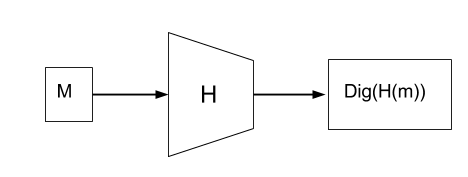
\includegraphics[scale=0.4]{images/10-hash}
  \caption{Model for hashing a message}
\end{figure}

\textbf{The ideal Hash function} has 4 main properties:
\begin{itemize}
\item It is easy to compute the hash value for any given message
\item It is infeasible to generate a message that has a given hash (pre-image)
\item It is infeasible to modify a message without changing the hash
\item It is infeasible to find two different messages with the same hash (collision)
\end{itemize}

\textbf{Security of Hash functions}

% \textbf{Private key:}

% \textbf{Private key:}

\subsection{Birthday paradox}
Probability of finding a collision. Given a function $f$ that maps
values to $H$ different outputs, the probability of finding a
collision after $n$ randomly selected inputs is

\[ p(n; H) \approx 1 - e^{\frac{-n(n-1)}{2H}} \approx 1 - e^{\frac{-n^2}{2H}} \]

This expression can be invertedto $n(p; H)$ describing how many tries
$n$ it takes to reach a probability $p$ of collision

\[ n(p; H) \approx \sqrt{2H \ln \frac{1}{1 - p}} \]

To achieve $0.5$ chance of collision this gives

\[ n(0.5; H) = 1.1774 \sqrt{H} \]

\textbf{Example:} For a 128 bit hash there are $2^{128}$ different
hashes, and the number of tries needed to achieve $0.5$ chance of
collision is then

\[ 1.1774 \sqrt{2^{128}} \approx 2.17 \cdot 10^{19} \]

\subsection{Complexity of collisions}

\subsection{Iterated Hash-functions}
A hash function must be able to process an arbitrary-length message
into a fixed-length output. This can be achieved by breaking the input
up into a series of equal-sized blocks, and operating on them in
sequence using a one-way compression function.

To make sure the message fits the blocks of the compression function,
we apply a padding function.

We will show that this provides a method for showing that if one finds
a collision for the hashing function, one also found a collision for
the compression function.

\begin{figure}[H]
  \begin{centering}
    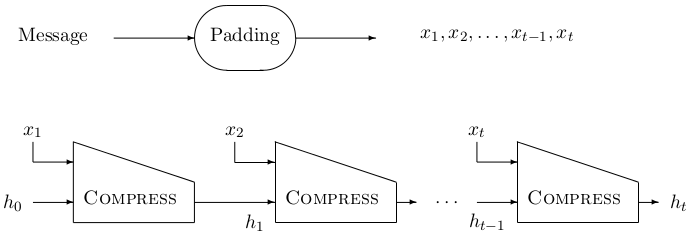
\includegraphics[width=12cm]{images/10-it-hash}
    \caption{Model of iterated hash-functions}
  \end{centering}
\end{figure}

\begin{figure}[H]
  \centering
  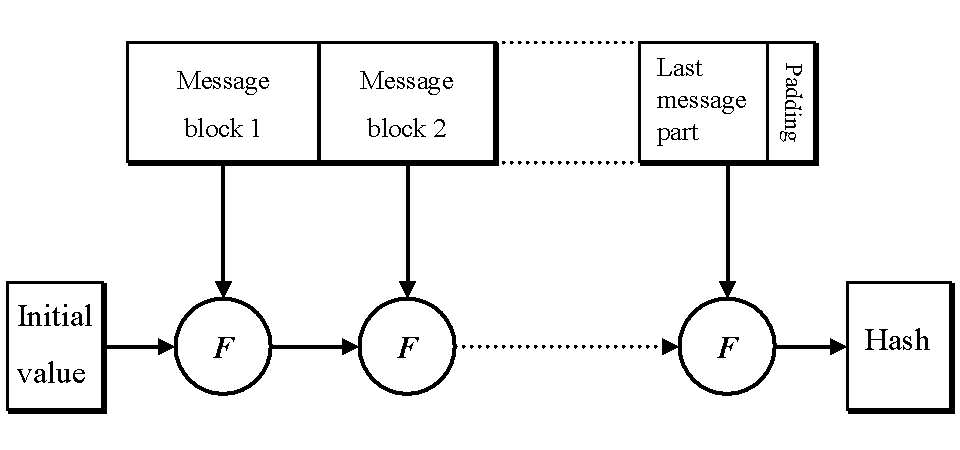
\includegraphics[scale=0.3]{images/10-padding}
  \caption{Model for hashing using padding}
\end{figure}

\subsection{The Merkle-Damgård Construction}
Let $h$ be a compression function:
\[ h: \{0,1\}^N \rightarrow \{0,1\}^n \quad \text{where } N > n \]

We construct a hash-function $H$, for some large value $M$:
\[ H: \{0,1\}^M \rightarrow \{0,1\}^n \]

\subsubsection*{Padding}
\begin{itemize}
\item Let $x \in \{0,1\}^v$ be a $v$-bit string to be hashed
\item First append a one-bit to $x$, that is, $x := x | ‘1’$. Now the length of $x$ is $v + 1$.
\item Let $s$ be the least positive integer such that $v + 1 + s +
  l_M$ is a multiple of $N - n$,\\ e.i. $s \equiv - (v + 1 + l_M) \mod
  (N-n)$
\item Append $s$ zero-bits to $x$.
\item Append to $x$ a block of $l-M$ bits which contains the binary representation of the integer
\end{itemize}

A hash function built with the Merkle–Damgård construction is as
resistant to collisions as is its compression function; any collision
for the full hash function can be traced back to a collision in the
compression function.